\documentclass[11pt]{article}
% Кодировка и язык
\usepackage[utf8]{inputenc}           % Кодировка исходного файла (UTF-8)
\usepackage[T2A]{fontenc}             % Кодировка шрифтов для кириллицы
\usepackage[english,russian]{babel}   % Локализация: русские названия, переносы

% Поиск в PDF
\usepackage{cmap}                     

% Поля страницы
\usepackage{geometry}
\geometry{left=2cm, right=2cm, top=2cm, bottom=2cm}

% Математика
\usepackage{amsmath, amssymb, amsthm} % Базовые пакеты для математики
\usepackage{mathtools}                % Расширение amsmath (доп. символы и окружения)

% Картинки
\usepackage{graphicx}                 % Вставка картинок (\includegraphics)
\graphicspath{{pictures/}}            % Путь к папке с картинками
\usepackage{float}                    % Позволяет использовать [H] для жёсткого позиционирования
\usepackage{wrapfig}                  % Обтекание текста вокруг картинок

% Таблицы
\usepackage{array}                    % Расширенные возможности для таблиц
\usepackage{booktabs}                 % Красивые таблицы (\toprule, \midrule, \bottomrule)
\usepackage{multirow}                 % Объединение строк в таблицах
\usepackage{tabularx}                 % Таблицы с автоматической шириной колонок
\usepackage{ragged2e}                 % Улучшенное выравнивание (используется в tabularx)

% Списки
\usepackage{enumitem}                 % Гибкая настройка списков (itemize, enumerate)

% Колонтитулы
\usepackage{fancyhdr}                 

% Гиперссылки
\usepackage{xcolor}                   % Работа с цветами
\usepackage{hyperref}                 % Гиперссылки, оглавление, перекрёстные ссылки

% Умные ссылки
\usepackage{cleveref}                 

% Типографика
\usepackage{microtype}                % Улучшает переносы и межсловные расстояния

% Подписи к картинкам и таблицам
\usepackage{caption}                  % Настройка подписей (шрифт, отступы)

% Рисование схем и графиков
\usepackage{tikz}                     % Рисование схем, графиков, диаграмм
\usepackage{pgfplots}                 % Построение графиков функций (на основе tikz)
\pgfplotsset{compat=newest}           % Версия совместимости pgfplots

% Алгоритмы и код
\usepackage{algorithm}                % Окружения для алгоритмов
\usepackage{algorithmic}              % Синтаксис для алгоритмов
\usepackage{listings}                 % Вставка кода с подсветкой синтаксиса


% Настройка нумерации секций и подсекций
\renewcommand{\thesection}{\arabic{section}}                   
\renewcommand{\thesubsection}{\thesection.\arabic{subsection}} 


% Настройка списков: убираем лишние отступы слева
\setlist[itemize]{leftmargin=}
\setlist[enumerate]{leftmargin=}


% Определение окружений для теорем, лемм, определений и т.д.
% Нумерация привязана к номеру секции
\newtheorem{theorem}{Теорема}[section]
\newtheorem{definition}{Определение}[section]
\newtheorem{remark}{Замечание}[section]
\newtheorem{lemma}{Лемма}[section]
\newtheorem{example}{Пример}[section]
\newtheorem{consequence}{Следствие}[section]
\newtheorem{algorithmm}{Алгоритм}
\newtheorem{question}{Вопрос}[section]
\newtheorem{answer}{Ответ}[section]
\newtheorem{statement}{Утверждение}[section]


% Определение цветов
\definecolor{pblue}{rgb}{0.13,0.13,1}    
\definecolor{pgreen}{rgb}{0,0.5,0}       
\definecolor{pred}{rgb}{0.9,0,0}         
\definecolor{pgrey}{rgb}{0.46,0.45,0.48}

\newcommand{\lectureNumber}{2}
\newcommand{\lectureTitle}{Законы динамики}
\newcommand{\courseName}{Цифровизация физических процессов}
\newcommand{\semester}{3 семестр, 2026/2027 уч. год}

\pagestyle{fancy}
\fancyhf{}
\fancyhead[L]{Это та часть, где ты убегаешь}
\fancyhead[R]{\thepage}
\setlength{\headheight}{15pt}

\hypersetup{
    colorlinks=true,
    linkcolor=blue!70!black,
    citecolor=blue!70!black,
    filecolor=blue!70!black,
    urlcolor=blue!70!black,
}

\begin{document}


\begin{titlepage}
    \centering
    
    {\large Московский физико-технический институт \par}
    {\large Высшая школа программной инженерии \par}
    \vspace{2cm}

    {\Large \textbf{\courseName} \par}
    {\large \semester \par}
    
    \vspace*{\fill}

    {\Huge \textbf{Лекция \lectureNumber} \par}
    {\Huge \textbf{\lectureTitle} \par}
    
    \vspace*{\fill}
    
    {\large Лектор: Попов Павел Владимирович  \par}
    {\large Автор: \href{https://t.me/mallina_olga}{\sout{когда-нибудь затехает это}} \par}

\end{titlepage}

\pagenumbering{arabic}

\section{Опыты Галилея}

\subsection{Опыт 1}
\begin{figure}[H]
    \centering
    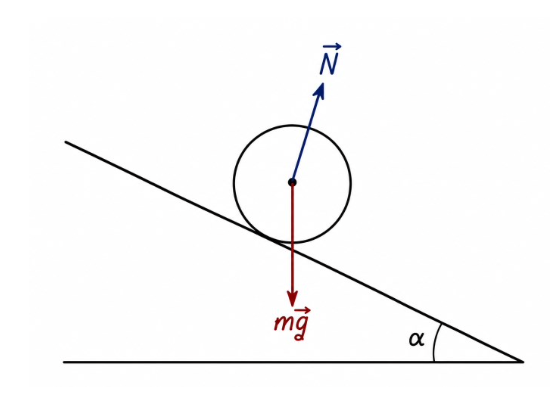
\includegraphics[width=0.4\linewidth]{1 опыт.png}
\end{figure}
Для опыта Галилей взял шар, движущийся по наклонной плоскости. Рассмотрим силы, действующие на этот шар.
Есть сила тяжести, которая имеет проекцию вдоль плоскости, которая определяется углом $\alpha$. Также есть сила реакции опоры, которая направлена перпендикулярно наклонной плоскости, поэтому её проекция на направление вдоль плоскости равна 0. 
Поэтому движение вдоль плоскости будет определяться только проекцией $m\vec{g}$ на это направление. Теперь проведём измерение и попытаемся понять, является ли скорость постоянной. Заметим, что при измерении получаем постоянное ускорение при постоянной силе. Тогда получаем следующее соотношение: 
\[ F \sim a \] 
Но так как мы хотим получить закон, то имеем
\[ \vec{F} = m\vec{a} =  m \frac{d^2\vec{r}}{dt^2} \]

\subsection{Опыт 2}

\begin{figure}[H]
    \centering
    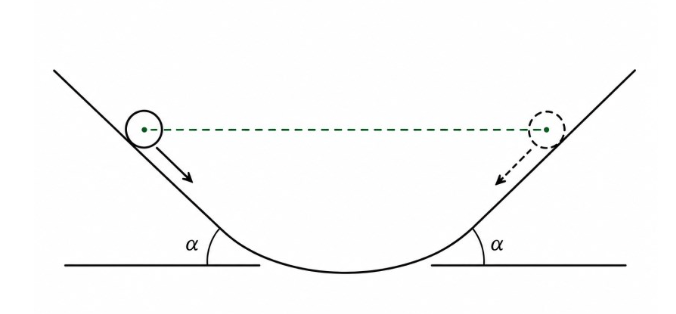
\includegraphics[width=0.4\linewidth]{2 опыт.png}
\end{figure}

Галилей поставил 2 желоба напротив друг друга и заметил, что если пустить шар с какой-то высоты одного желоба, то шар поднимется примерно на ту же высоту второго желоба, с которой начинал движение, за вычетом небольшой потери на трение. 
При отсутствии трения шар, спустившись с одной высоты, должен подняться по второму желобу до той же высоты. При уменьшении угла наклона второго желоба для достижения той же высоты ему потребуется пройти всё больший путь.
Тогда у него возникла потрясающая мысль поставить один желоб горизонтально (продолжение в 3 опыте). 




\subsection{Опыт 3}
\begin{figure}[H]
    \centering
    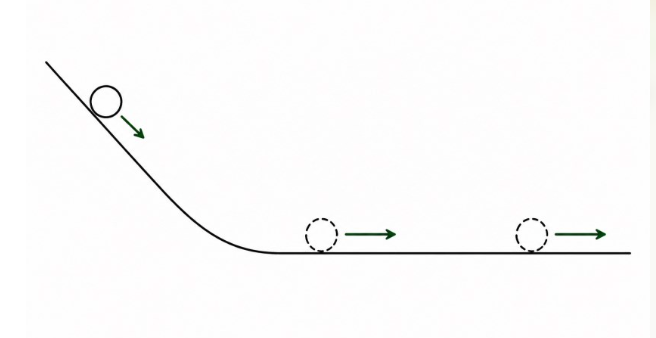
\includegraphics[width=0.4\linewidth]{3 опыт.png}
\end{figure}

Галилей поставил 1 желоб под наклоном, а второй горизонтально. Далее он пустил шарик по наклонному желобу и стал измерять зависимость пройденного расстояния от времени по горизонтальному желобу. Получив линейную зависимость, он сделал вывод о том, что при отсутствии трения шарик будет двигаться бесконечно с постоянной скоростью. 


\section{Третий закон Ньютона}

\begin{figure}[H]
    \centering
    \includegraphics[width=0.5\linewidth]{третий закон ньютона.png}
\end{figure}

Рассмотрим систему из двух точек, изолированную от других тел. На первую точку действует сила $\vec{F}_{21}$,  а на вторую --- $\vec{F}_{12}$.
Теперь, посмотрев на эту систему со стороны с достаточно большого расстояния, можно рассмотреть её как материальную точку. 
Тогда, получим, что 
\[ \vec{F}_{12} = - \vec{F}_{21} \] 
Далее обобщим эту систему до $n$ точек. Тогда полную силу взаимодействия, действующую на какую-то из точек, можно представить как сумму сил попарного взаимодействия с остальными телами системы. 
Тогда верно следующее:
\[ \vec{F}_{ik} = - \vec{F}_{ki} \] 

Более того 
\[ \vec{F}_{ik} || \vec{r} _{ik} \]  

\begin{remark}
    Последнее утверждение $(\vec{F}_{ik} || \vec{r} _{ik})$  справедливо только в классической механике. 
\end{remark}


\section{Законы динамики}

\subsection{Принцип инерции}
Тело покоится или двигается с постоянной скоростью, если на него не действуют силы или действие сил скомпенсировано.

\begin{definition}
    Система отсчёта, в которой свободное тело покоится или двигается равномерно и прямолинейно, называется \textbf{инерциальной}. 
\end{definition}


\begin{itemize}
    \item \textbf{Импульс тела} изменяется при взаимодействии с другими телами, то есть в результате действия сил.
    \item \textbf{Ускорение} определяется взаимодействием тела с другими телами, то есть действующими силами. 
\end{itemize}


\subsection{Закон сохранения импульса}
\begin{figure}[H]
    \centering
    \includegraphics[width=0.5\linewidth]{третий закон ньютона.png}
\end{figure} 

Рассмотрим две изолированные точки, которые взаимодействуют друг с другом. Вспомним, что такое импульс:
\[ \vec{p} = m\vec{v} \Rightarrow \frac{d\vec{p}}{dt}  = m\frac{d\vec{v}}{dt} = m\frac{d^2\vec{r}}{dt^2} \]   
Запишем полный импульс системы:
\[ \vec{p} = \vec{p_1} + \vec{p_2} \]

\[ \frac{d\vec{p}}{dt} = \frac{d\vec{p_1}}{dt} + \frac{d\vec{p_2}}{dt} = \vec{F}_{21} + \vec{F}_{12} \Rightarrow \vec{p}= const\]  

Конечно же закон справедлив не только для двух точек. Поэтому получим: импульс системы остаётся неизменным при равенстве нулю геометрической суммы внешних сил.


\section{Кинетическая энергия}

\subsection*{Элементарная работа}Для того чтобы дать определение кинетической энергии нам необходимо вспомнить, что такое работа:

\begin{figure}[H]
    \centering
    \includegraphics[width=0.3\linewidth]{картинка с работой.png}
\end{figure} 

\[ dA = \vec{F}\cdot d\vec{r} \text{     (здесь имеется в виду скалярное произведение)} \]

\[ dA = F_xdx+ F_ydy + F_zdz \]
\begin{figure}[H]
    \centering 
    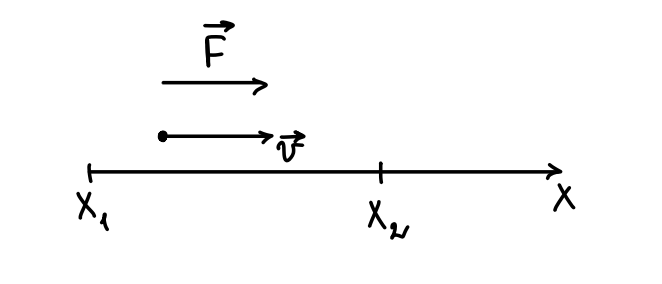
\includegraphics[width=0.5\linewidth]{картиночка для понимания 1.png}
\end{figure} 

\[ A_{12} = \int_{1}^{2} Fdx = \int_{1}^{2} \frac{dp}{dt}\,dx = \int_{1}^{2} dp \frac{dx}{dt} = \int_{v_1}^{v_2} mv\,dv = \frac{m{v_2}^2}{2} - \frac{m{v_1}^2}{2} \] 




Работа может быть равна нулю, даже если сила ненулевая. Это
происходит, например, когда сила перпендикулярна перемещению:
магнитное поле действует на заряженную частицу и закручивает
её движение, но работы не совершает. Другой случай — отсутствие
перемещения: можно долго толкать стену, однако механическая работа
при этом не совершается.


Итого получим: 
\[ K = \frac{mv^2}{2} \text{--- кинетическая энергия } \] 
 


\subsection*{Теорема о кинетической энергии}
\begin{figure}[H]
    \centering 
    \includegraphics[width=0.5\linewidth]{теорема о кинетической энергии.png}
\end{figure} 
\[ A_{12} = K_2 -K_1 \text{ --- теорема о кинетической энергии } \]   


\subsection*{Столкновения}
При столкновении тела могут разойтись или слипнуться. Если
кинетическая энергия сохраняется, удар называют абсолютно упругим.
При неупругом ударе часть энергии переходит во внутреннюю энергию:
тела деформируются и нагреваются. В предельном случае абсолютно
неупругого удара вся доступная кинетическая энергия переходит
во внутреннюю энергию, а тела после столкновения движутся вместе.
\begin{figure}[H]
    \centering 
    \includegraphics[width=0.4\linewidth]{неупругий удар.png}
\end{figure} 


\begin{figure}[H]
    \centering 
    \includegraphics[width=0.4\linewidth]{упругий удар.png}
\end{figure}

Рассмотрим абсолютно упругое столкновение двух тел c массами \(m_1\) и \(m_2\), 
которые до столкновения движутся со скоростями $v_1$ и $v_2$. 
После столкновения их скорости становятся равными $v_1'$ и $v_2'$.

\begin{figure}[H]
    \centering 
    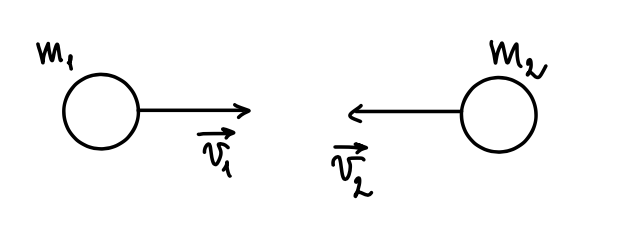
\includegraphics[width=0.4\linewidth]{шарики в столкновениях.png}
\end{figure}

Поскольку удар абсолютно упругий, сохраняются одновременно импульс системы и её кинетическая энергия. Поэтому можно записать систему: 
\[ \begin{cases}
    m_1v_1+ m_2v_2 = m_1v_1'+ m_2v_2'\\
    \frac{m_1v_1^2}{2} + \frac{m_2v_2^2}{2} = \frac{m_1v_1'^2}{2} + \frac{m_2v_2'^2}{2}\\
    \end{cases} \] 
Решим эту систему, получим: 
\[ v_1' = -v_1 +2\frac{m_1v_1+m_2v_2}{m_1+m_2} \]
\[ v_2' = -v_2 +2\frac{m_1v_1+m_2v_2}{m_1+m_2} \] 
Рассмотрим частный случай, когда $ m_1 = m_2, v_2 =0$. Тогда из полученных выше формул следует:  
\[ v_1' = -v_1+v_1 =0 \]
\[ v_2' = 0+v_1 = v_1 \]   

Теперь рассмотрим случай, когда $v_2=0$, а $m_2=\frac{1}{10}m_1$:
\[ v_1' = -v_1+2\frac{m_1v_1}{m_1+\frac{1}{10}m_1} = -v_1 + \frac{20}{11}v_1 = \frac{9}{11}v_1 \]   
\[ v_2' = 0 + 2\frac{m_1v_1}{m_1+\frac{1}{10}m_1} = \frac{20}{11} v_1 \] 



\section{Классификация сил}

\subsection*{Консервативные силы}
\begin{definition}
    \[ A = \oint \vec{F}\, \cdot d\vec{l} = 0 \]
    \begin{itemize}
        \item сила гравитационного взаимодействия
        \item сила Кулона
        \item сила упругости
        \item + силы, сводящие к центральным
    \end{itemize}
\end{definition}

\subsection*{Не консервативные силы}

\begin{definition}
   \[ A = \oint \vec{F}\, \cdot d\vec{l} \neq 0 \]
   \begin{itemize}
    \item сила трения во всех проявлениях
   \end{itemize}
\end{definition}


\end{document}